\documentclass[../main.tex]{subfiles}
\graphicspath{{\subfix{../images/}}}

\begin{document}

\subsection{Γενική Περιγραφή}
\begin{enumerate}
	\item Οι οντότητες είναι ο \textbf{Χαρακτήρας} (character), ο \textbf{οίκος}
	      (house), τα μη ανθρώπινα \textbf{έμβια όντα} (non human) τα οποία είναι
	      είτε ζωώδη πλάσματα (beast) είτε φυτοειδή (plants), η \textbf{θρησκεία}
	      (religion), και τα \textbf{σημαντικά γεγονότα} στην μυθοπλασία του Game Of Thrones
	      (notable events) .
	\item Για κάθε χαρακτήρα έχουμε πολλές συνδέσεις υποχρεωτικές και μη. Ο
	      χαρακτήρας είναι πιθανό να ανήκει σε έναν οίκο αλλά ένας οίκος είναι
	      υποχρεωτικό να αποτελείται από αυτούς.
	\item Επίσης μπορεί να έχει ένα μη ανθρωποειδές ων στην κατοχή του ή να
	      πιστεύει σε μια θρησκεία.
	\item Δεν είναι υποχρεωτικό να έχει συμμετάσχει σε ένα σημαντικό γεγονός αν
	      και αυτό είναι το πιο πιθανό γιατί κάποια από αυτά θα μπορεί ας πούμε να
	      συνέβησαν μόνο με δράκους (beast).
\end{enumerate}

% ------Table template for entities-------
\newcommand{\entityTable}[4]{
	\renewcommand{\arraystretch}{1.5}
	\tymin 0.25\textwidth
	\begin{table}[H]
		\centering
		\begin{tabulary}{\textwidth}{R|L}
			\hline
			\multicolumn{2}{c}{Οντότητα: \textbf{#1}} \\
			\hline
			\textbf{Περιγραφή}  & #2  \\
			\textbf{Ιδιότητες}  & #3  \\
			\textbf{Γνωρίσματα} & #4  \\
			\hline
		\end{tabulary}
		\caption{Οντότητα #1}
	\end{table}
}

% ------Table template for relations-------
\newcommand{\relationTable}[6]{
	\renewcommand{\arraystretch}{1.5}
	\tymin 0.3\textwidth
	\begin{table}[H]
		\centering
		\begin{tabulary}{\textwidth}{R|L}
			\hline
			\multicolumn{2}{c}{Συσχέτιση: \textbf{#1}} \\
			\hline
			\textbf{Περιγραφή}            & #2  \\
			\textbf{Ιδιότητες}            & #3  \\
			\textbf{Λόγος πληθικότητας}   & #4  \\
			\textbf{Συμμετοχή}            & #5  \\
			\textbf{Γνωρίσματα}           & #6  \\
			\hline
		\end{tabulary}
		\caption{Συσχέτιση \texttt{#1}}
	\end{table}
}

\subsection{Καθορισμός Οντοτήτων}

\entityTable{Character}
{Οντότητα που αποθηκεύονται οι χαρακτήρες}
{Ισχυρή Οντότητα}
{character\_id, name, date\_of\_birth, date\_of\_death, culture, titles}

\entityTable{house}
{Οντότητα που αποθηκεύονται οι οίκοι}
{Ισχυρή Οντότητα}
{house\_name, slogan, location}

\entityTable{non\_human}
{Οντότητα που αποθηκεύονται τα μη ανθρώπινα έμβια πλάσματα}
{Ισχυρή Οντότητα, Υποκλάσεις: Beast, Plants}
{name, species, ID}

\entityTable{notable\_events}
{Οντότητα που αποθηκεύονται τα σημαντικά γεγονότα}
{Ισχυρή Οντότητα}
{nickname, date, locations, type\_of\_event, outcome}

\entityTable{religion}
{Οντότητα που αποθηκεύονται οι θρησκείες}
{Ισχυρή Οντότητα}
{name}

\entityTable{beast}
{Οντότητα που αποθηκεύονται τα ζωώδη πλάσματα}
{Ασθενής οντότητα του non\_human}
{domestic}

\entityTable{plant}
{Οντότητα που αποθηκεύονται τα φυτά}
{Ασθενής οντότητα του non\_human}
{}

\entityTable{location}
{Οντότητα που αποθηκεύονται οι τοποθεσίες}
{Ισχυρή Οντότητα}
{name, x, y}

\subsection{Καθορισμός Συσχετίσεων}

\relationTable{character\_belongs\_to\_house}
{Κάθε χαρακτήρας μπορεί να έχει έναν οίκο τον οποίο υπηρετεί.}
{belongs-to: διαδική}
{N:1}
{Μερική Συμμετοχή του Character \newline Ολική συμμετοχή του House}
{-}

\relationTable{Friends}
{Κάθε χαρακτήρας μπορεί να έχει έναν φίλο ο οποίος είναι πάλι character}
{Αναδρομική-recursive}
{N:M}
{Ολική συμμετοχή του character}
{-}

\relationTable{Relatives}
{Κάθε χαρακτήρας μπορεί να έχει έναν συγγενή ο οποίος είναι πάλι character}
{Αναδρομική-recursive}
{N:M}
{Ολική συμμετοχή του character}
{-}

\relationTable{house\_leadership\_character}
{Κάθε οίκος πρέπει να έχει κάποια ηγεσία}
{leadership: δυαδική}
{1:Ν}
{Ολική συμμετοχή του house \newline Μερική συμμετοχή του character}
{-}

\relationTable{Notable\_event\_happened\_in\_location}
{Κάθε σημαντικό γεγονός πρέπει να έχει συβεί σε μία τοποθεσία}
{happened\_in: δυαδική}
{Ν:1}
{Μερική συμμετοχή του location \newline Ολική συμμετοχή του notable\_events}
{-}

\relationTable{House\_is\_at\_location}
{Κάθε οίκος πρέπει να είναι σε κάποια τοποθεσία}
{is\_at: δυαδική}
{1:1}
{Μερική συμμετοχή του location \newline Ολική συμμετοχή του House}
{-}

\relationTable{character\_owns\_non\_human}
{Κάθε χαρακτήρας μπορεί να έχει έμβυα πλάσματα στην κατοχή του. }
{owns\_a: δυαδική}
{N:M}
{Μερική Συμμετοχή του Character \newline Μερική Συμμετοχή του Non human}
{-}

\relationTable{character\_has\_religion}
{Κάθε χαρακτήρας μπορεί να έχει μία ή και παραπάνω θρησκείες.}
{owns\_a: δυαδική}
{N:M}
{Μερική Συμμετοχή του Character \newline Μερική Συμμετοχή του Non human}
{-}

\relationTable{character\_participates\_in\_notable\_events}
{Κάθε χαρακτήρας μπορεί να συμμετεχει σε ένα σημαντικό γεγονός.}
{participates\_in: δυαδική}
{N:M}
{Μερική Συμμετοχή του Character \newline Ολική Συμμετοχή του notable events}
{-}

\relationTable{Non\_human\_is\_a\_beast/plant}
{Κάθε non human μπορεί να είναι είτε ζωώδες πλάσα είτε φυτό.}
{is\_a: προσδιορίζουσα }
{1:1}
{Ολική συμμετοχή του Non\_human \newline Ολική Συμμετοχή του beast/plant }
{-}

\subsection{Διάγραμμα Οντοτήτων/Συσχετίσεων}

\begin{figure}[H]
	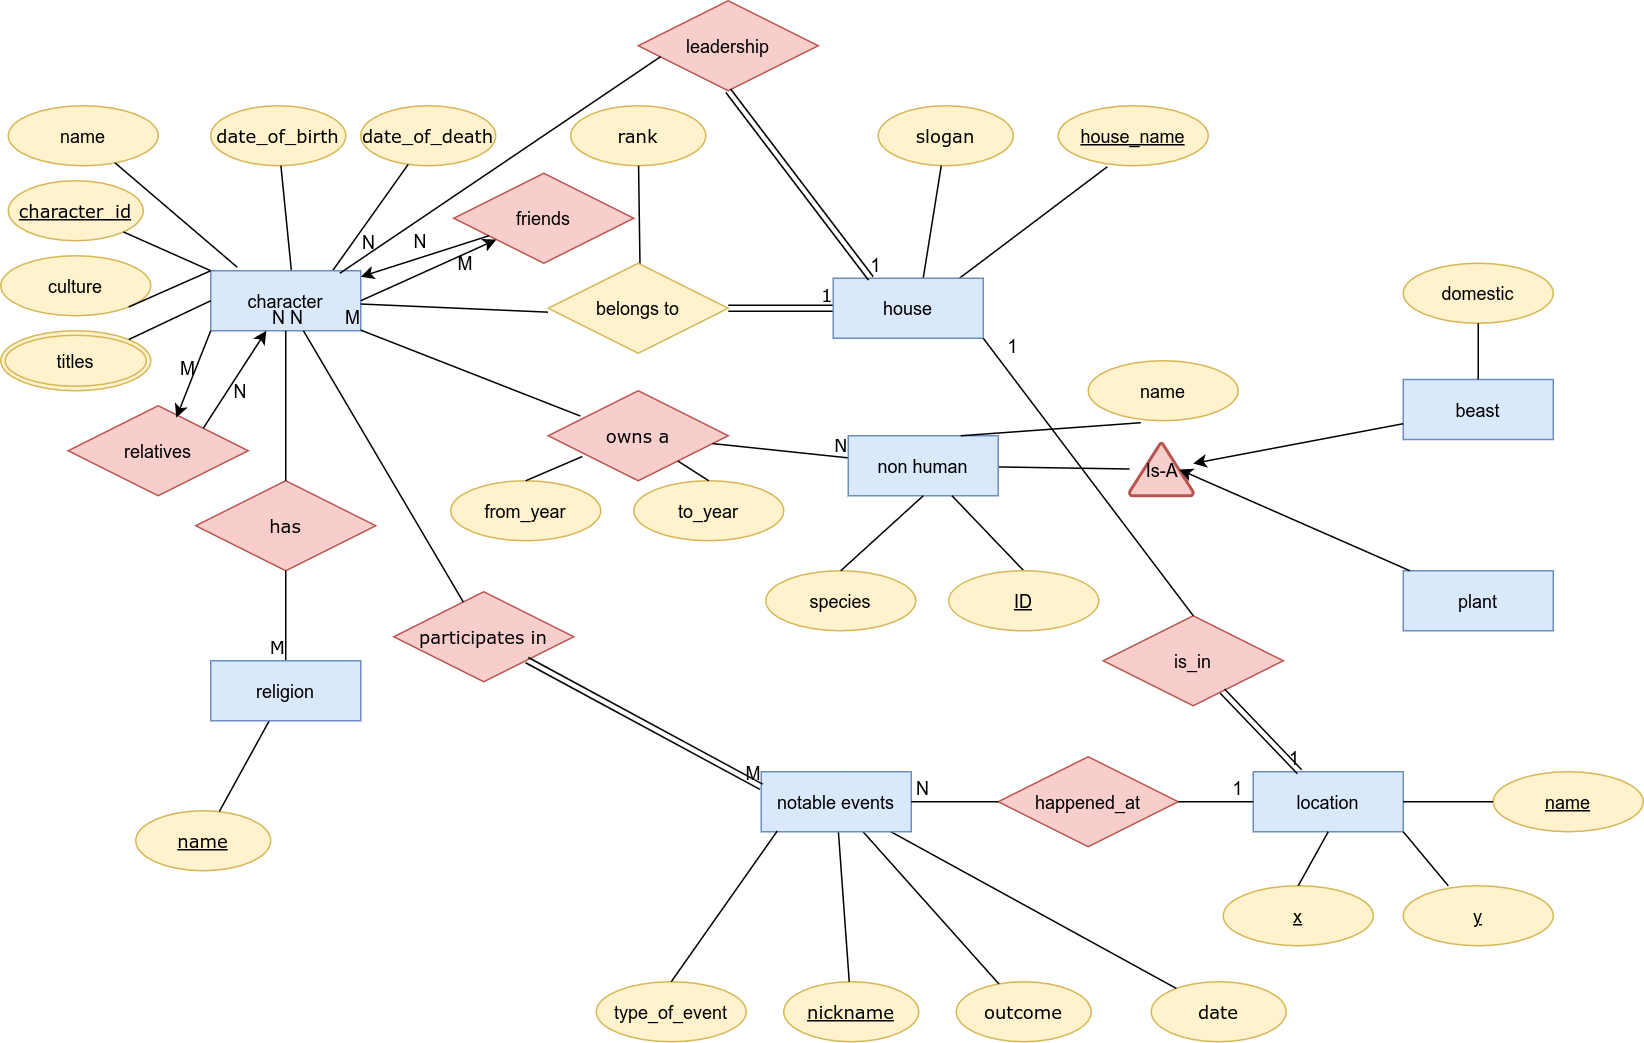
\includegraphics[width=\textwidth]{../images/entity_relation_diagram.png}
	\caption{Διάγραμμα Οντοτήτων/Συσχετίσεων}
\end{figure}


\end{document}
